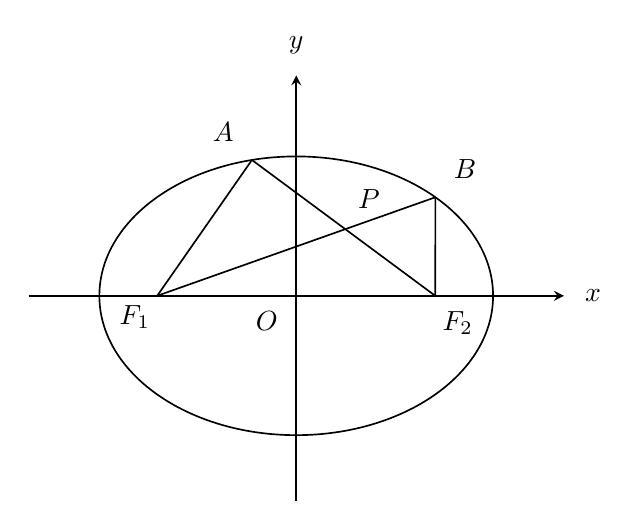
\begin{tikzpicture}[x=1cm,y=1cm,line width=.6pt]
% ellipse x^2/2+y^2=1 scaled: rx=2.5, ry=1.77; F at +-1.77
\coordinate (O) at (0,0);
\coordinate (F1) at (-1.7655310816,0.0000000000);
\coordinate (F2) at (1.7655310816,0.0000000000);
\coordinate (A) at (-0.5623776359,1.7246350147);
\coordinate (B) at (1.7677669530,1.2515790027);
\coordinate (P) at (0.6233387678,0.8461950604);
\draw[-stealth] (-3.4,0)--(3.4,0) node[right,xshift=4pt] {$x$};
\draw[-stealth] (0,-2.6)--(0,2.8) node[above,yshift=4pt] {$y$};
\draw (0,0) ellipse (2.5 and 1.77);
\draw (A)--(F1) (A)--(F2);
\draw (B)--(F2) (B)--(F1);
\node[below left,xshift=1pt,yshift=0pt] at (F1) {$F_{1}$};
\node[below right,xshift=-1pt,yshift=-2pt] at (F2) {$F_{2}$};
\node[below left,xshift=-3pt,yshift=-2pt] at (O) {$O$};
\node[above left,xshift=-3pt,yshift=3pt] at (A) {$A$};
\node[above right,xshift=3pt,yshift=3pt] at (B) {$B$};
\node[above right,xshift=1pt,yshift=4pt] at (P) {$P$};
\end{tikzpicture}
